
\chapter{Related Work\label{ch:pastwork}}

\section{Quadcopters for Model Acquisition}

	The past decade has seen a huge increase in the use of quadcopters for a variety of applications. With the improvement of stabilization software, quadcopters have seen a rise in popularity as a stable, cheap, and highly maneuverable aerial platform. 

	Although a relatively new field, several research groups have studied the use of quadcopters in 3D model construction. Irschara et al. created a system to generate 3D models using images taken from UAVs. While a quadcopter was used for gathering imagery, the quadcopter was manually controlled and the main focus of their work was photogrammetry-based model creation \cite{Irschara}. Steffen et al. studied surface reconstruction using aerial photography captured by UAVs \cite{Steffen}.

	 \begin{figure}[ht]
            \centering
            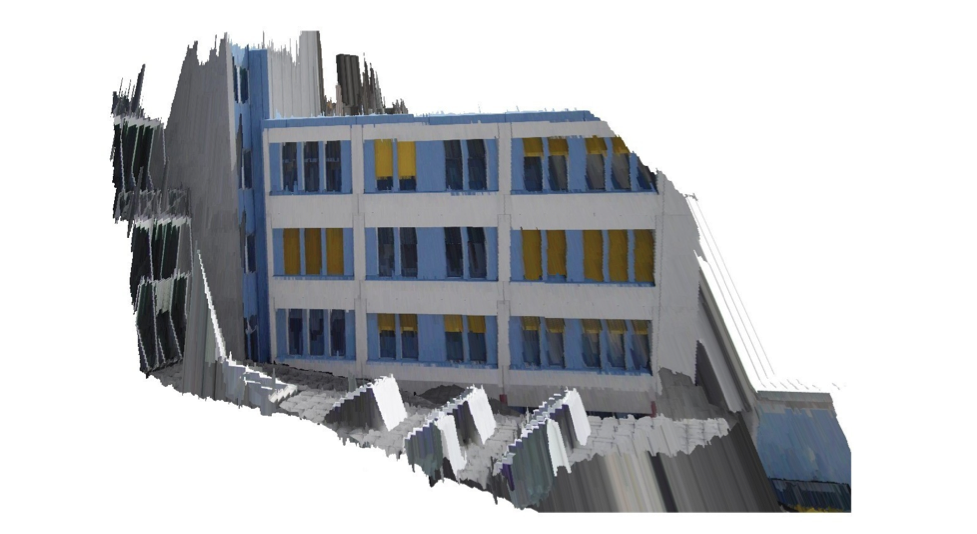
\includegraphics[width=300px]{../images/Irschara.png}
            \caption{3D Model of Building By Irschara et al.~\cite{Irschara}}\label{fig:Irschara}
    \end{figure}

	Most relevant to this project, Engel et al. have published multiple papers on the camera-based navigation and localization of the AR.Drone~\cite{Engel, Engel2}. While they were able to achieve very accurate navigation, their work relies on the drone facing a mostly planar surface during the entire flight. As constructing models requires capturing imagery from a variety of positions and headings, this constraint is not acceptable.

	\begin{figure}[ht]
            \centering
            \begin{subfigure}[b]{0.5\textwidth}
                    \centering
                    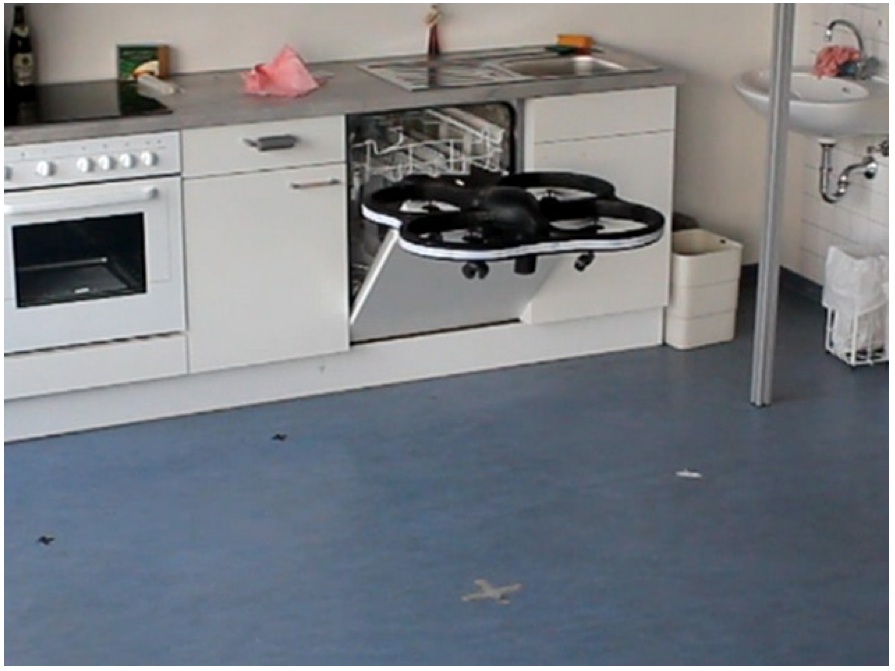
\includegraphics[width=0.8\textwidth]{../images/Engel2.png}
                    \caption{Flying environment}
            \end{subfigure}%
            ~ %add desired spacing between images, e. g. ~, \quad, \qquad etc.
              %(or a blank line to force the subfigure onto a new line)
            \begin{subfigure}[b]{0.5\textwidth}
                    \centering
                    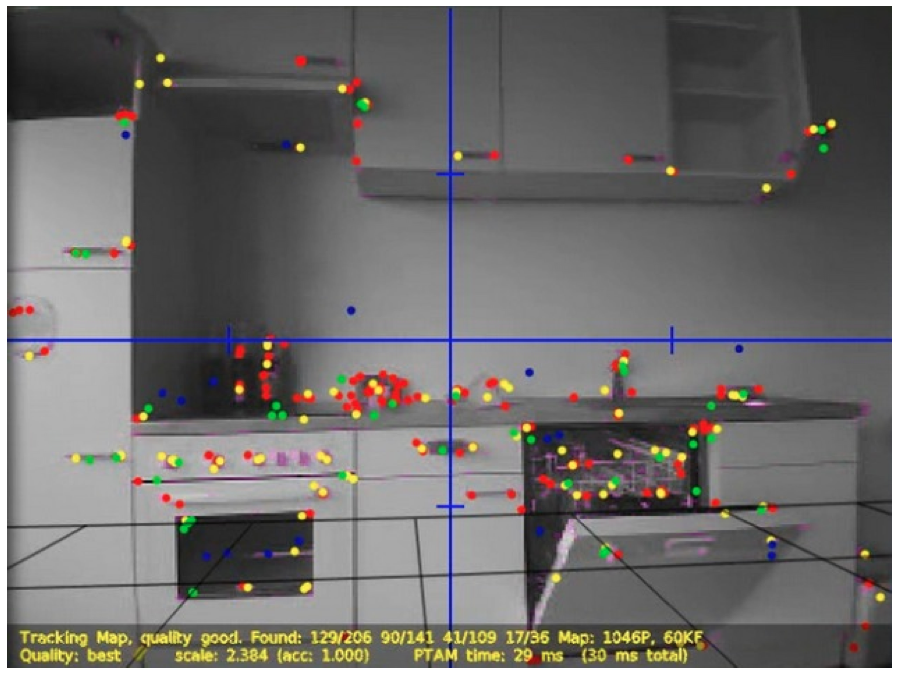
\includegraphics[width=0.8\textwidth]{../images/Engel1.png}
                    \caption{Camera view with detected features}
            \end{subfigure}
            \caption{AR.Drone Localization Using Monocular SLAM~\cite{Engel2}.}
    \end{figure}


\section{GPS-denied Navigation of Quadcopters}

	There has been substantial work done on autonomous navigation of quadcopters without the use of GPS. As GPS signal cannot typically penetrate the walls or ceilings, any autonomous flights taking place indoors must use methods other than GPS for localization. Most of these methods rely on using vanishing point detection in order to navigate hallways and other interior spaces.

	\begin{figure}[ht]
            \centering
            \begin{subfigure}[b]{0.5\textwidth}
                    \centering
                    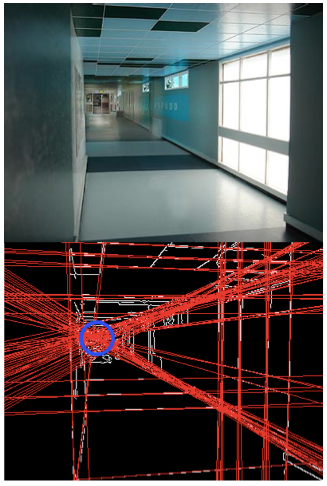
\includegraphics[width=0.8\textwidth]{../images/Bills1.png}
                    \caption{Vanishing point detection}
            \end{subfigure}%
            ~ %add desired spacing between images, e. g. ~, \quad, \qquad etc.
              %(or a blank line to force the subfigure onto a new line)
            \begin{subfigure}[b]{0.5\textwidth}
                    \centering
                    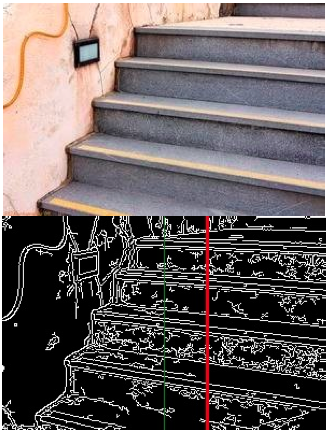
\includegraphics[width=0.8\textwidth]{../images/Bills2.png}
                    \caption{Stair detection}
            \end{subfigure}
            \caption{Localization Using Perspective Cues~\cite{Bills}.}
    \end{figure}

	Bills et al. present a method for navigating in an unknown interior space with the AR.Drone. By performing edge detection on the forward and downward facing cameras, their algorithm is able to determine the type of environment the quadcopter is in, either hallway or staircase, and issues the appropriate commands to autonomously navigate the space~\cite{Bills}. While this system is a great step in exploring interior space, it does not provide a solution to our problem. Unlike the work by Bills et al., our system must operate in essentially open space, with few visual cues such as vanishing point available for reference.

